\documentclass[a4paper]{llncs}
\usepackage{amsmath}

\usepackage{tikz}
\usetikzlibrary{positioning}
\usetikzlibrary{calc}
\usetikzlibrary{arrows,shapes,backgrounds}

\newcommand{\vphi}{\vec{\varphi}}
\newcommand{\vi}{{\vec{i}}}
\newcommand{\vj}{{\vec{j}}}
\newcommand{\vmu}{\vec{\mu}}

\title{ GPU-accelerated and CPU SIMD Optimized \\ Monte Carlo Simulation of $\phi^4$ Model}
\author{Piotr Bialas \and Jakub Kowal \and Adam Strzelecki}
\institute{Faculty of Physics, Astronomy and Applied Computer Science\\
Jagiellonian University\\
ul. Reymonta 4, 30-059 Krakow, Poland }
\begin{document}


\maketitle


This contribution is concerned with an efficient implementation of the
Monte-Carlo simulations of the $\varphi^4$ model\cite{parisi}. The
problem is defined as follows: having a vector field $\vphi$ defined
on a regular rectangular two or three dimensional grid we want to
generate the field configurations with probability proportional to
$\exp(-H(\vphi))$ where $H(\vphi)$ is some function of all the fields
$\vphi_i$.

The actual generation is done by the mean of the Metropolis
algorithm. This amounts to sequentially updating all the points of
the lattice. The crucial feature of this algorithm is that the update
is local {\em i.e.} The new value of the field in a given point
depends only on the values of fields in the immediate neighborhood of
the updated point. In our case this neighborhood is extended
compared to usual nearest neighbors (see figure~\ref{fig:nn}
(Right)). The update is random and requires a good source of
pseudo-random numbers. We use the  Tausworthe RNG\cite{howes_thomas07}.



While model is inherently parallelizable, grid points that lie in
the same neighborhood cannot be updated together. Taking into
account a larger neighborhood means that a simple checkerboard
decomposition pattern cannot be used and we have devised a new grid
decomposition scheme.
\begin{figure}
\begin{center}
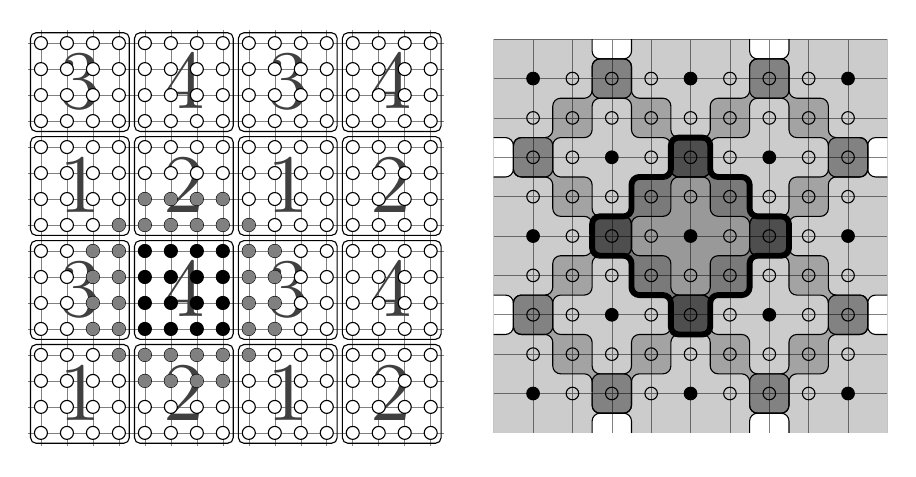
\begin{tikzpicture}[scale=0.5]
\begin{scope}[scale=0.66]
\draw[very thin, gray] (-0.5,-0.5) grid (15.5,15.5);

\foreach \x in {0,8}
\foreach \y in {0,8}
\draw[xshift=\x cm, yshift = \y cm]
node[darkgray,scale=3] at (1.5cm,1.5) {$1$}
node[darkgray,scale=3] at (5.5cm,1.5) {$2$}
node[darkgray,scale=3] at (1.5cm,5.5) {$3$}
node[darkgray,scale=3] at (5.5cm,5.5) {$4$} ;

\foreach \x in {0,...,15}
 \foreach \y in {0,...,15} {
  \fill[white] (\x, \y) circle(0.25);
  \draw[black] (\x, \y) circle(0.25);
}

\foreach \x in {4,...,7}
  \foreach \y in {4,...,7}
    \fill[black] (\x, \y) circle(0.25);

\foreach \x in {4,...,7}
  \foreach \y in {2,3,8,9}
    \fill[gray] (\x, \y) circle(0.25);

\foreach \x in {2,3,8,9}
  \foreach \y in {4,...,7}
    \fill[gray] (\x, \y) circle(0.25);

\foreach \p in {(3,3),(3,8),(8,3),(8,8)}
  \fill[gray] \p circle(0.25);

\foreach \x in {0,4,...,12}
  \foreach \y in {0,4,...,12}
    \draw[black,xshift=\x cm, yshift=\y cm, rounded corners = 2pt] (-.4,-0.4)
      rectangle (3.4cm,3.4cm);

\end{scope}

\begin{scope}[xshift=14.5cm,yshift=3cm]
\clip (-3,-3) rectangle (7,7);

\draw[help lines] (-3.0,-3.0) grid (7.0,7.0);

% lattice points
\foreach \x in {-2,-1,0,1,2,3,4,5,6}
  \foreach \y in {-2,-1,0,1,2,3,4,5,6}
    \draw (\x,\y) + (0.0,0.0) circle (0.16);

% neighborhood
\foreach \p in {(-2.5,4.0),(1.5,4.0),
                (-2.5,0.0),(1.5,0.0),
                (-4.5,2.0),(3.5,2.0),
                (-4.5,6.0),(-0.5,6.0),(3.5,6.0),
                (-4.5,-2.0),(-0.5,-2.0),(3.5,-2.0)
            }
  \path[draw=black,fill, fill opacity=0.20,rounded corners=0.1cm,shorten >=2pt]
    \p-- ++(0,-0.5)-- ++(1,0)-- ++(0,-0.5)-- ++(0,-0.5)-- ++(1,0)--
    ++(0,-1.0)-- ++(1,0)-- ++(0,1.0)-- ++(1,0)-- ++(0,1.0)-- ++(1,0)--
    ++(0,1)-- ++(-1,0)-- ++(0,1)-- ++(-1,0)-- ++(0,1)-- ++(-1,0)-- ++(0,-1)--
    ++(-1,0)-- ++(0,-1)-- ++(-1,0)-- ++(0,-0.6);

% main center neighborhood

\path[draw=black,fill,fill opacity=0.4,rounded corners=0.1cm,shorten >=2pt,line width=0.75mm,cap=round,join=round]
  (-0.5,2.0)-- ++(0,-0.5)-- ++(1,0)-- ++(0,-0.5)-- ++(0,-0.5)-- ++(1,0)--
  ++(0,-1.0)-- ++(1,0)-- ++(0,1.0)-- ++(1,0)-- ++(0,1.0)-- ++(1,0)--
  ++(0,1)-- ++(-1,0)-- ++(0,1)-- ++(-1,0)-- ++(0,1)-- ++(-1,0)-- ++(0,-1)--
  ++(-1,0)-- ++(0,-1)-- ++(-1,0)-- ++(0,-0.6);

\fill[black] (-2,2) circle(0.16);
\fill[black] (2,2) circle(0.16);
\fill[black] (6,2) circle(0.16);
\fill[black] (0,4) circle(0.16);
\fill[black] (0,0) circle(0.16);
\fill[black] (4,0) circle(0.16);
\fill[black] (4,4) circle(0.16);
\fill[black] (-2,-2) circle(0.16);
\fill[black] ( 2,-2) circle(0.16);
\fill[black] ( 6,-2) circle(0.16);
\fill[black] (-2,6) circle(0.16);
\fill[black] ( 2,6) circle(0.16);
\fill[black] ( 6,6) circle(0.16);


\end{scope}

\end{tikzpicture}
\end{center}
\caption{\label{fig:nn} (Left) The partition of the lattice into
  blocks. The blocks with same number are processed in parallel by
  different thread blocks.  (Right) Partitioning of the blocks into
  disjoint sublattices.  Thick black line denotes the neighborhood  used in updating the center point. Black points are processes in parallel by
  different threads of the same thread block.}
\end{figure}


% GPU implementation
On GPU we adopt the hierarchical scheme from ref.~\cite{weigel}
suitably modified to account for bigger neighborhood.  We first divide
the whole lattice in blocks of $32\times 32$ points. Then we start a
kernel that process every forth block (see figure~\ref{fig:nn}).  Each
block is assigned to a block of 128 threads. First we fetch the values of the fields from global to shared memory (including border points).  
After that each thread updates
one point from the first partition. Then after synchronization, next
partition is updated and so on. After processing all eight(2D) or 16
(3D) partitions the kernel writes the shared memory back into global
and new kernel is started processing next batch of blocks. 
Altogether in this
way we managed to achieve $0.13$ nanoseconds for single lattice field
update on \emph{NVIDIA GTX 470}, reaching around $430$ Gflops that is
$40\%$ of $1088$ Gflops peak performance of this device .

% CPU implementation
In order to provide unbiased CPU vs GPU speed up results we provide
multithreaded vectorized CPU implementation. It uses OpenMP for
parallel execution, CPU SSE/AVX and compiler vector extensions for
vectorization.  This implementation does mimic GPU SIMT execution
model.  The SIMD instructions are used to process four (SSE) or eight
(AVX) updates in parallel. We use partitions as on CPU but we use only
one level {\em i.e.} we do not partition the lattice into blocks.
However not all scalar \emph{x86} instructions have vector
counterparts.  In particular direct \emph{XMM} registers gather and
scatter and vectorized integer operations for full length AVX 256-bit
registers are missing, which makes impossible to port random number
generator from 128-bit SSE to 256-bit AVX. Initially planned for AVX
standard, these were postponed to AVX2 planned for 2013. As soon AVX2
capable CPU devices appear on the market we plan to revise our
evaluation.


Our CPU \emph{OpenMP} and \emph{SSE/AVX} implementation compiled via
GCC 4.4 or higher and running on \emph{Intel Core i5 2.5 Ghz} quad
core CPU presented $15\times$ performance boost comparing to single
threaded scalar code and $3.76$ nanoseconds for single lattice field
update.  Which gives the $15$ Gflops that is $\sim10\%$ of the  $160$
Gflops peak performance of tested i5 CPU. There is no significant
increase in performance while switching from SSE to AVX instructions.

This gives around $28\times$ advantage to GPU, which is noticeably
less than promised by many publications, however much higher that
comes from comparison of  tested i5
CPU to \emph{GTX 470}. This can be
traced back to 128-bit only \emph{Tausworthe} random number generator
implementation and inefficient vector store and load operations
(gather/scatter).

\begin{thebibliography}{9}
\bibitem{parisi} G.~Parisi ``Statistical Field Theory'' Chapter 5, Perseus Books Publishing (1998).
\bibitem{weigel} M.~Weigel, J. Comput. Phys. \textbf{231}, 3064 (2012).
\bibitem{howes_thomas07}
Lee Howes and David Thomas.
``{\em Efficient random number generation and application using {CUDA}.}''
In Hubert Nguyen, editor, {\em GPU Gems 3}, chapter~37. Addison
  Wesley, August 2007.
\end{thebibliography}

\end{document}
